\chapter{Revisão de Literatura}

\par
As abordagens que buscam realizar previsões no mercado financeiro utilizam inúmeros conceitos na composição de seus modelos, e tangem inúmeras áreas do conhecimento, tais como: estatística, mercado financeiro, economia e computação. Historicamente, há também diferentes formas de análise no que diz respeito a tomada de decisão no mercado financeiro, que também serão apresentadas. Abaixo estão separados subtópicos referentes a conceitos importantes para a literatura de Séries Temporais Financeiras.

\subsection{\textbf{Mercado de Ações}}

\par
O conceito de Ação representa uma fração do capital social de uma empresa quaisquer, ou seja, títulos que são vendidos em diferentes níveis de participação para compor uma sociedade investidora. O mercado de ações representa essa forma das empresas de obter capital que posteriormente é aplicado em recursos que possibilitará o crescimento desta, e consequentemente no lucro dos compradores através da distribuição de dividendos. Os investidores têm a expectativa de lucrar com empresas que geram lucro e se valorizam. O valor das ações é volátil, sofre influência de inúmeras direções, tais como as leis do mercado, a lei da oferta e procura, fatores macroeconômicos, notícias, taxas e juros bancários, decisões dos investidores \cite{chenZhao13}. Seguem abaixo alguns atributos respectivos a ações, usualmente utilizados para exemplificá-las, também presentes em gráficos do mercado financeiro, conjuntos de dados e afins:

\begin{itemize}
\item{\textit{Open}}: Preço de abertura; corresponde ao preço da primeira negociação do período.
\item{\textit{High}}: Preço máximo; corresponde ao maior valor alcançado no período.
\item{\textit{Low}}: Preço mínimo; corresponde ao valor mais baixo do período.
\item{\textit{Close}}: Preço de fechamento; corresponde ao valor da última negociação do período.
\item{\textit{Volume}}: Volume; é o total de ações negociadas durante o período.
\end{itemize}

\par
Tais atributos apresentados estão presentes nos indicadores financeiros, utilizados vastamente pelos analistas a fim de procurar e entender padrões no mercado. \cite{2006technical}.

\subsection{\textbf{Métodos de Análise e Previsão de Ações}}

\par A previsão de ações ou movimentos na bolsa de valores ocorre quando as séries temporais extraídas não seguem \textit{random walks} - movimentos aleatórios e imprevisíveis, portanto não passíveis de previsão \cite{jason} - \cite{castelao}

\subsubsection{Análise Técnica}

\par
Análise que se baseia nas forças que regem as decisões dos investidores, criando uma dinâmica com os valores passados, projetando-os para o futuro mediante análise de gráficos e da utilização de indicadores. Ignora fatores externos e foca nas mudanças das ações, na tentativa de prever anomalias e movimentos. Dentre os indicadores utilizados, podemos citar: indicadores de filtro, indicadores de volume, indicadores de momento, entre outros \cite{castelao}.

\subsubsection{Análise Fundamentalista}

\par
A análise fundamentalista se baseia nos fatores micro e macroeconômicos de uma empresa para inferir a respeito da dinâmica do mercado de ações. Analisa os fatores humanos, os setores e a organização interna de uma empresa, seu estado atual, suas relações e os fatores externos. Possui a vantagem de poder realizar previsões antes mesmo destas aparecerem nos gráficos, bem como a desvantagem de automatizar devido a complexidade e subjetividade das análises \cite{castelao}.

\subsubsection{Séries Temporais}

\par
Por fim, temos as séries temporais, de nosso interesse para esse relatório. Séries Temporais são séries em que as observações apresentam uma dependência sequencial, de forma que em um tempo \textit{t}, as observações $\textit{t}-1$, $\textit{t}-2$ em diante apresentam influência nos valores futuros. Séries Temporais são conjuntos dessas observações com intervalos regulares de tempo \cite{jason}.

\par
Podemos também destacar os componentes característicos de uma séries temporal\footnote{\href{https://www.maxwell.vrac.puc-rio.br/4244/4244_5.PDF}{Análise de Séries Temporais: PUC-Rio}. Acesso em 14 mai. 2021.}:

\begin{itemize}
    \small
    \item{\textit{tendência}: indica seu comportamento ``a longo prazo'', bem como sua velociade de mudança.}
    \item{\textit{ciclo}: oscilação de subida e descida na série, de forma repetitiva e característica.}
    \item{\textit{sazonalidade}: osiclações de subida e descida caracterísitcas associadas a períodos específicos, como por exemplo períodos do ano.}
\end{itemize}

\subsection{\textbf{Previsão em Séries Temporais}}

\par
Tipicamente, um conjunto de dados da bolsa de valores apresenta a característica de ser separado por unidades de tempo, usualmente em dias, tal qual uma ação fecha o dia com um determinado preço que é denominado de “\textit{close}”. No estudo de estatística e mineração de dados, uma série numérica com essa característica temporal, separada em períodos, é denominada de série temporal. Séries temporais podem ser obtidas de inúmeras aplicações científicas, em fenômenos da natureza e em aplicações financeiras. Dentre os exemplos de Séries temporais, pode-se destacar: eletrocardiogramas, temperaturas diárias, vendas semanais de produtos, bolsa de valores, entre outros. No tocante às características das Séries temporais, os dados podem estar distribuídos de forma sazonal ou aleatória. A Série pode ainda ser estacionária ou não estacionária. As abordagens da análise de Séries temporais buscam a extração de informações do passado para estudar comportamentos futuros através dos métodos de análise e da aplicação dos modelos de predição, identificando padrões diversos \cite{fu2011}. Seguem abaixo alguns modelos estatísticos de predição de dados utilizados em séries temporais:

\begin{itemize}
\item{Modelo de Médias Móveis (\textit{Moving Average} ou MA)}
\item{Modelo Autorregressivo (\textit{Autoregressive model} ou AR)}
\item{Modelo Autorregressivo de Médias Móveis (\textit{Autoregressive-moving-average} ou ARMA)}
\item{Modelo Autorregressivo Integrado de Médias Móveis (\textit{Autoregressive integrated moving average} ou ARIMA)}
\end{itemize}

\subsubsection{Modelo Autorregressivo (\textit{Autoregressive Model} ou AR)}

O modelo Autorregressivo é utilizado para realizar previsões em Séries Temporais, utilizando observações passadas em uma equação regressiva para prever os valores futuros. O modelo AR é uma combinação linear de valores, passados como \textit{input}, que geram \textit{outputs} tratados como previsões da série \cite{jason}. Este modelo pertence à família de modelos estatísticos tradicionais para a previsão em séries temporais; por ser robusto, foi utilizado neste trabalho para trazer uma base comparativa. O modelo Autorregressivo de ordem \textit{p}, AR(\textit{p}), se dá pela equação abaixo\footnote{Disponível em: \href{http://www.portalaction.com.br/series-temporais/41-modelos-autorregressivos-ar}{Portal Action: Modelos Autorregressivos}. Acesso em 13 mai. 2021.}:

\begin{equation}
X_{t}=k+\sum _{{i=1}}^{p}\varphi _{i}X_{{t-i}}+\varepsilon _{t}\,
\end{equation}

Onde $\mathrm{\varphi_{1}}$,\ ..\ .\ ,\ $\mathrm{\varphi_{n}}$ são os parâmetros do modelo, \textit{k} é uma constante e $\mathrm{\varepsilon_t}$ é o ruído branco. 

\subsection{\textbf{Previsão em Séries Temporais Financeiras}}
 \par
A partir das técnicas de análise de Séries Temporais Financeiras, podemos extrair padrões característicos, tais como sazonalidade, ciclos, tendência e caminhada aleatória. Os padrões extraídos usualmente são combinados a técnicas específicas de mineração de dados, tais como associação, agrupamento, classificação, sumarização e regressão \cite{fu2011}. Como mencionado, as Séries Temporais podem ainda ser estacionárias, ou então não estacionárias, como é o caso das séries provenientes da bolsa de valores. As estacionárias flutuam entorno de uma mesma média ao longo do tempo, em contrapartida das não estacionárias \cite{fu2011}. Na análise das características de uma série do mercado de ações, há períodos que podem conter tendências, ciclos e caminhadas aleatórias (random walks) ou então uma combinação um ou mais desses três elementos. A previsão em séries temporais do mercado de ações, portanto, é essencialmente dinâmica, não linear, complexa, não paramétrica e caótica \cite{abuMostafaAtiya96}.

\subsection{\textbf{Aprendizagem de Máquina (\textit{Machine Learning})}}

\par
Como mencionado anteriormente, a abordagem de \textit{Machine Learning} vem utilizando técnicas para realizar previsões em séries temporais. Em aprendizagem de máquina, podemos citar algumas formas distintas de aprendizado:

\begin{itemize}
    \item{Aprendizagem supervisionada}
    \item{Aprendizagem não supervisionada}
    \item{Aprendizagem semi-supervisionada}
    \item{Aprendizagem por reforço}
\end{itemize}

\par
Podemos citar, no que tange a aprendizagem supervisionada, as técnicas de aprendizagem profunda \textit{Deep Learning}, dos quais utilizaremos as técnicas CNN e LSTM neste relatório.

\subsubsection{Aprendizagem Profunda (\textit{Deep Learning})}

\par
As técnicas de aprendizagem profunda são eficazes em realizar o aprendizado por meio de representações computacionais de elementos diversos, como imagens, músicas e afins. Essas representações simples geram processos de aprendizagem extremamente complexos \cite{GoodBengCour16}. Os tópicos abaixo tratam de duas técnicas de \textit{Deep Leanrnig} que serão utilizadas neste relatório.

\subsubsubsection{\textit{Rede Neural Convolucional} (\textit{Convolutional Neural Network} ou CNN)}

\par
A técnica CNN é especializada em processamento de dados em topologia de grade, como pode ser o caso das Séries Temporais (de nosso interesse), através dos dados passados como uma grade de uma dimensão, em intervalos regulares \cite{GoodBengCour16}.


%---------------FIGURE
\begin{figure}[H]
\centering
\caption{Representação de uma rede convolucional (CNN).}
  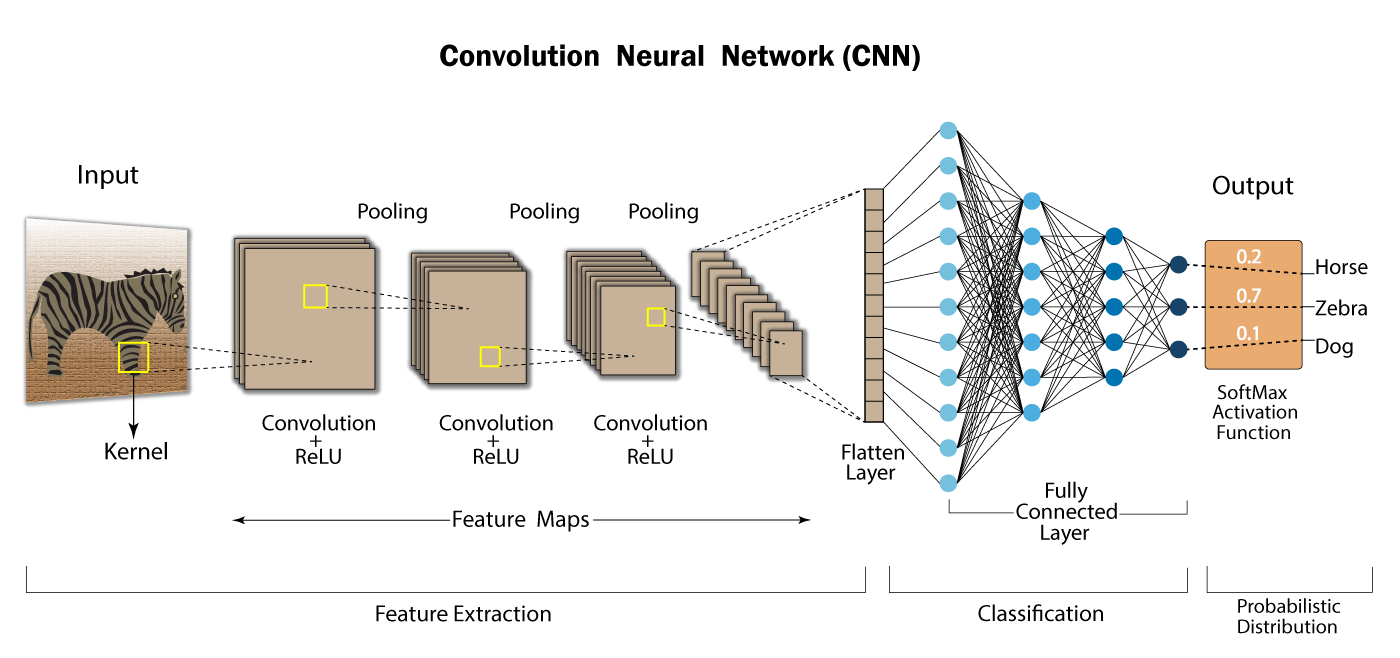
\includegraphics[scale=0.33]{figures/cnn_banner.png}
  Fonte: \href{https://developersbreach.com/convolution-neural-network-deep-learning/}{Developers Breach}. Acesso 13 de mai. 2021.
\end{figure}


\subsubsubsection{\textit{Memória de Longo e Curto Prazo} (\textit{Long Short-Term Memory} ou LSTM)}

\par
As LSTMs são redes neurais recorrentes, e foram introduzidas por Hochreiter \& Schmidhuber (1997). Possuem uma vasta aplicação em inúmeras áreas e são extensamente utilizadas no mercado financeiro \cite{castelao}. A técnica LSTM também apresenta resultados eficientes nas áreas de reconhecimento de voz, reconhecimento de dígitos escritos à mão, entre outros \cite{GoodBengCour16}.

%---------------FIGURE
\begin{figure}[hbt]
\centering
\caption{Representação de uma unidade LSTM, com componentes estruturais e operações matemáticas.}
  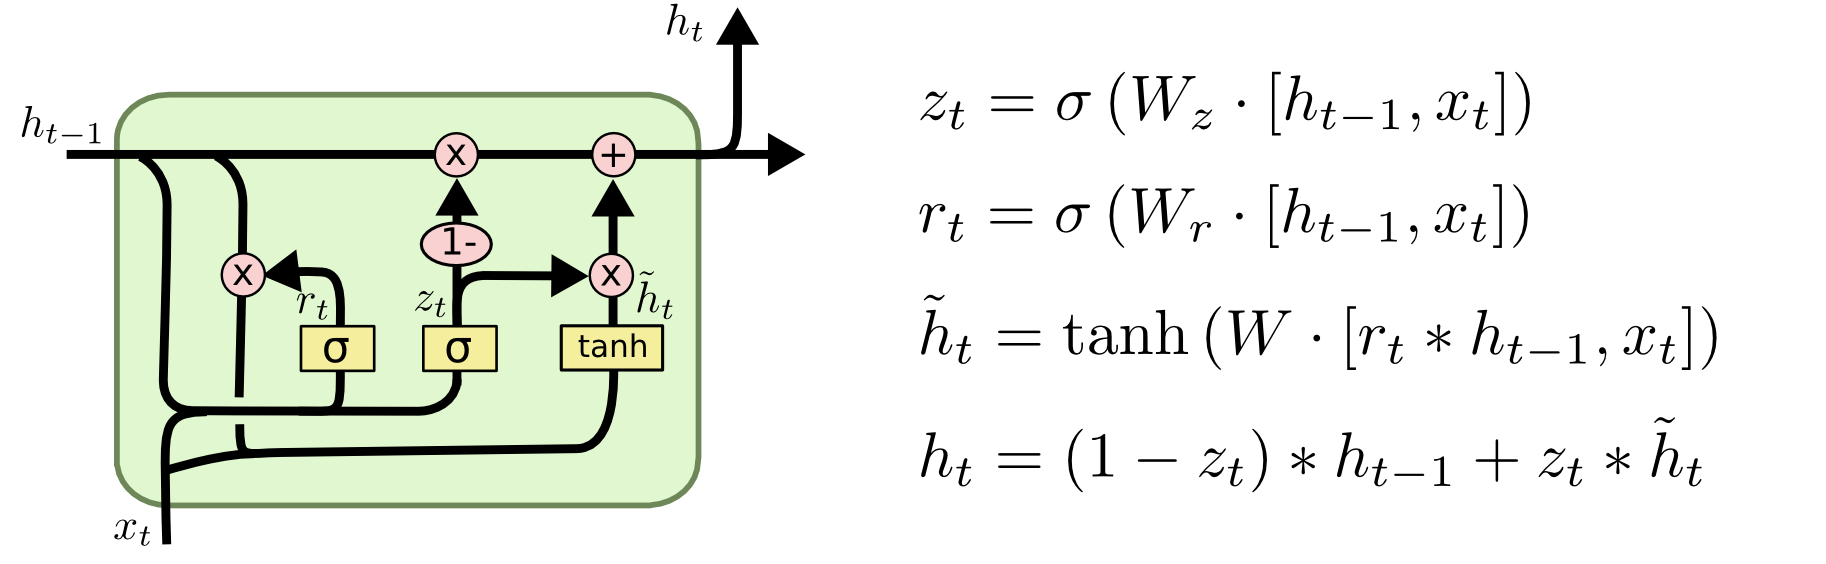
\includegraphics[scale=0.56]{figures/lstm.png} \\
  Fonte: \href{http://colah.github.io/posts/2015-08-Understanding-LSTMs/}{Colah's Blog}. Acesso 13 de mai. 2021.
\end{figure}